% ============================================================
%  PFZ Navigator — IEEE Conference Paper (IEEEtran format)
%  Authors: Harshath Mukundan, Praveen N
%  Institution: SRM Institute of Science and Technology
% ============================================================
\documentclass[conference]{IEEEtran}
\usepackage[utf8]{inputenc}
\usepackage{amsmath,amssymb,amsfonts}
\usepackage{graphicx}
\usepackage{textcomp}
\usepackage{xcolor}
\usepackage{booktabs}
\usepackage{multirow}
\usepackage{array}
\usepackage{cite}
\usepackage{hyperref}
\usepackage{float}
\usepackage{subcaption}
\usepackage{tikz}
\usetikzlibrary{shapes.geometric, arrows.meta, positioning, fit, calc}

% Custom column types
\newcolumntype{C}[1]{>{\centering\arraybackslash}p{#1}}

% TikZ styles for architecture diagrams
\tikzstyle{block} = [rectangle, rounded corners, minimum width=2.8cm,
    minimum height=0.7cm, text centered, draw=black, font=\footnotesize]
\tikzstyle{inputblock} = [block, fill=blue!15]
\tikzstyle{encblock} = [block, fill=cyan!20]
\tikzstyle{bottleneck} = [block, fill=orange!25]
\tikzstyle{decblock} = [block, fill=green!15]
\tikzstyle{outblock} = [block, fill=red!15]
\tikzstyle{arrow} = [thick,->,>=stealth]
\tikzstyle{skiparrow} = [thick,->,>=stealth, dashed, color=gray]

\begin{document}

\title{PFZ Navigator: Deep Learning-Based Geospatial\\
Decision Support System for Potential Fishing Zone\\
Identification Using U-Net and ConvLSTM}

\author{
\IEEEauthorblockN{Praveen N}
\IEEEauthorblockA{Dept.\ of Computing Technologies\\
SRM Institute of Science and Technology\\
Kattankulathur, Chennai, India\\
pn7054@srmist.edu.in}
\and
\IEEEauthorblockN{Dr S Praveena}
\IEEEauthorblockA{Dept.\ of Computing Technologies\\
SRM Institute of Science and Technology\\
Kattankulathur, Chennai, India\\
praveens@srmist.edu.in}
\and
\IEEEauthorblockN{R S Harshath Mukundan}
\IEEEauthorblockA{Dept.\ of Computing Technologies\\
SRM Institute of Science and Technology\\
Kattankulathur, Chennai, India\\
rs5485@srmist.edu.in}
}

\maketitle

% ============================================================
%                        ABSTRACT
% ============================================================
\begin{abstract}
Accurate identification and forecasting of Potential Fishing
Zones (PFZs) is essential for sustainable fisheries management
and fuel-cost reduction for coastal fishing communities along
the Tamil Nadu coastline. Existing advisory systems issued
by agencies such as INCOIS employ threshold-based gradient
analysis on Sea Surface Temperature (SST) and Chlorophyll-a
imagery, limiting their capacity to capture nonlinear multi-
parameter interactions that govern fish aggregation. This paper
presents~\textbf{PFZ Navigator}, an end-to-end geospatial decision
support system that integrates two complementary deep learning
architectures --- a \textbf{U-Net} encoder-decoder network for high-
resolution spatial segmentation of current-day PFZ boundaries,
and a \textbf{Convolutional LSTM (ConvLSTM)} network for seven-day
spatio-temporal PFZ forecasting --- trained on multi-channel
CMEMS satellite oceanography data comprising SST, Sea Surface
Height (SSH), $u$/$v$-currents, and Chlorophyll-a, regridded to a
$256 \times 256$ standardised grid ($5^\circ$N--$14.5^\circ$N,
$77^\circ$E--$84.92^\circ$E). Temporal Block 3-fold cross-validation
for U-Net and Walk-Forward Expanding Window 3-fold
cross-validation for ConvLSTM enforce strict temporal separation
to prevent data leakage. The U-Net achieves~\textbf{92.13\%}
accuracy, \textbf{90.16\%} macro F1, Cohen's $\kappa = 0.849$,
and mIoU of~\textbf{82.29\%}. The ConvLSTM achieves
\textbf{88.49\%} accuracy, \textbf{88.32\%} macro F1,
$\kappa = 0.797$, and mIoU of~\textbf{79.24\%}. The system is
deployed as a full-stack web application with an interactive
Leaflet-based geographic dashboard featuring automated GPS
coordinate extraction and CSV export.
\end{abstract}

\begin{IEEEkeywords}
Potential Fishing Zone, U-Net, ConvLSTM, CMEMS, Semantic
Segmentation, Spatio-Temporal Forecasting, Cross-Validation,
Sea Surface Temperature, Chlorophyll-a, Deep Learning
\end{IEEEkeywords}

% ============================================================
%               I. INTRODUCTION
% ============================================================
\section{Introduction}

The fishing industry constitutes a critical pillar of the socio-economic
fabric of coastal communities in India, particularly along the
1,076~km Tamil Nadu coastline bordering the Bay of Bengal. Small-scale
and artisanal fishermen routinely navigate 20--80~km offshore,
consuming considerable quantities of diesel fuel to locate productive
fishing grounds through experiential knowledge alone. The Indian
National Centre for Ocean Information Services (INCOIS) provides
periodic Potential Fishing Zone advisories derived primarily from
satellite-observed SST fronts and Chlorophyll-a bloom boundaries
\cite{solanki2003}. These advisories rely on threshold-based rules
applied to only two oceanographic variables, failing to capture the
synergistic effects of multiple physical and biological forcing
mechanisms that collectively drive nutrient transport and plankton
aggregation \cite{tang2003}.

Several machine learning approaches have been applied to this domain.
Zhang et al.\ \cite{zhang_ensemble2023} employed ensemble classifiers
(Random Forest, SVM, XGBoost) on multi-parameter ocean data, achieving
86.92\% accuracy. Fitrianah et al.\ \cite{fitrianah2015} applied
spatio-temporal data mining with KNN classification on SST and
Chlorophyll, reaching 87.11\%. While these methods demonstrate the
value of multi-parameter inputs, they are fundamentally limited by
their inability to perform pixel-level spatial segmentation or temporal
forecasting of dynamic ocean fronts.

Deep learning has enabled substantial improvements. Sivasankari et
al.\ \cite{sivasankari2022} proposed HE-DFNETS, a hybrid CNN-LSTM
architecture for PFZ classification, and Vinston Raja et
al.\ \cite{vinston2023} applied Function Fitting Neural Networks for
daily PFZ forecasting. However, neither system offers pixel-wise
segmentation at the $256 \times 256$ spatial resolution necessary for
drawing geographic boundaries of fishing zones.

This paper presents \textbf{PFZ Navigator}, a dual-model deep learning
system that addresses two complementary operational requirements:
(1)~\emph{spatial analysis} of the current ocean state to generate
high-resolution PFZ maps (U-Net), and (2)~\emph{temporal forecasting}
of future PFZ distributions up to seven days ahead (ConvLSTM). The
principal contributions are:

\begin{itemize}
    \item A \textbf{multi-parameter deep learning pipeline} ingesting
    five co-registered oceanographic variables (SST, SSH, $u$-current,
    $v$-current, Chl-a) regridded to a unified $256 \times 256$ domain.
    \item A \textbf{U-Net encoder-decoder} with batch normalisation and
    skip connections for pixel-wise three-class PFZ segmentation,
    achieving \textbf{92.13\%} accuracy.
    \item A \textbf{ConvLSTM forecasting network} processing seven-day
    sequences to predict future PFZ maps, achieving \textbf{88.49\%}
    accuracy.
    \item \textbf{Rigorous temporal cross-validation protocols} (Temporal
    Block and Walk-Forward) preventing data leakage from auto-correlated
    satellite observations.
    \item A \textbf{full-stack decision support dashboard} with Leaflet
    geographic visualisation and automated GPS coordinate export.
\end{itemize}

% ============================================================
%               II. RELATED WORK
% ============================================================
\section{Related Work}

\subsection{Threshold-Based PFZ Advisory Systems}

The operational PFZ advisory framework deployed by INCOIS detects
oceanographic fronts through gradient thresholds applied to
satellite-derived SST and ocean colour (Chlorophyll-a) imagery
\cite{solanki2003}. Solanki et al.\ demonstrated that SST frontal
gradients serve as reliable proxies for fish aggregation in the
Arabian Sea. However, these threshold-based approaches consider only
two variables and are incapable of modelling the nonlinear multi-
parameter interactions that govern plankton blooms, upwelling dynamics,
and mesoscale eddy transport. Furthermore, they provide only current-
day snapshots and lack forecasting capability.

\subsection{Ensemble Machine Learning for PFZ Prediction}

Zhang et al.\ \cite{zhang_ensemble2023} employed ensemble machine
learning models --- Random Forest, SVM, KNN, and XGBoost --- on multi-
parameter oceanographic data including SST, Chlorophyll-a, latitude,
and longitude. Feature importance analysis revealed that Chlorophyll
and SST are the dominant predictors, and the ensemble approach
achieved an overall accuracy of 86.92\%. While this work confirms the
value of multi-parameter inputs, the ensemble framework treats each
location as an independent tabular sample and cannot produce pixel-
level spatial segmentation maps. Janani et al.\ \cite{janani2025}
extended this paradigm by combining clustering with ensemble
classification over seven ocean parameters, but similarly lack spatial
resolution and forecasting capability.

\subsection{Spatio-Temporal Data Mining Approaches}

Fitrianah et al.\ \cite{fitrianah2015} proposed a spatio-temporal data
mining framework for PFZ identification using SST and Chlorophyll
features processed through clustering and KNN classification. The
system achieved 87.11\% accuracy on historical catch records mapped to
satellite observations. A subsequent study by the same group
\cite{fitrianah_feature2016} investigated the effect of adding
salinity and current features, demonstrating improved prediction
accuracy with expanded input dimensionality. While these studies
validate the utility of spatio-temporal analysis, both rely on
traditional ML classifiers that produce coarse spatial predictions
incapable of delineating the fine-grained boundaries of thermal fronts
and upwelling zones.

\subsection{Deep Learning for PFZ Identification}

Sivasankari et al.\ \cite{sivasankari2022} proposed HE-DFNETS, a
hybrid deep learning framework combining CNN for spatial feature
extraction with LSTM for temporal modelling. The system achieved very
high classification accuracy ($\sim$99\%) on SST and Chlorophyll
inputs. While HE-DFNETS demonstrates the power of hybrid
architectures, it operates on extracted features rather than full
spatial grids, does not employ pixel-level semantic segmentation, and
lacks interpretability through geographic mapping. Our work extends
this paradigm by applying U-Net to full $256 \times 256$ spatial
grids for pixel-wise classification.

\subsection{Neural Network-Based PFZ Forecasting}

Vinston Raja et al.\ \cite{vinston2023} applied a Function Fitting
Neural Network (FFNN) to predict PFZ from 13 oceanographic features
including SST and Chlorophyll. The system targets daily forecasting
but lacks spatial modelling entirely --- each prediction is a scalar
classification rather than a spatial map. Our ConvLSTM architecture
overcomes this limitation by simultaneously capturing spatial
correlations through convolutional kernels and temporal dynamics
through recurrent gates, enabling full $256 \times 256$ spatial
forecasts up to seven days ahead.

\subsection{Convolutional LSTM for Spatio-Temporal Modelling}

Shi et al.\ \cite{shi2015} introduced the Convolutional LSTM
(ConvLSTM) architecture, which replaces the fully connected gates of
standard LSTM cells \cite{hochreiter1997} with convolutional
operations. Originally proposed for radar precipitation nowcasting,
ConvLSTM has since demonstrated state-of-the-art performance in tasks
requiring joint spatial and temporal modelling, including sea surface
temperature forecasting \cite{ham2019}. PFZ Navigator adopts ConvLSTM
for its unique ability to model moving ocean fronts and current-driven
advection patterns within a unified framework.

\subsection{U-Net for Semantic Segmentation}

Ronneberger et al.\ \cite{ronneberger2015} proposed the U-Net
encoder-decoder architecture with skip connections for biomedical
image segmentation. The architecture has become foundational in remote
sensing, where Zhang et al.\ \cite{zhang_unet2018} adapted it for
urban land cover classification. He et al.\ \cite{he2016} demonstrated
that residual skip connections improve deep network training by
preserving gradient flow. In PFZ Navigator, the U-Net skip connections
enable the decoder to preserve the high-resolution spatial boundaries
of thermal fronts and upwelling zones that are essential for accurate
GPS coordinate extraction.

\subsection{Review of PFZ Methodologies}

Ya'acob et al.\ \cite{yaacob2024} conducted a comprehensive review of
PFZ identification methodologies, cataloguing the features (SST, SSH,
Chlorophyll) and models (SVM, ANN, decision trees) used across the
literature. Their analysis identifies the lack of deep spatial
segmentation and temporal forecasting as major gaps in existing work
--- both of which are addressed by the dual-model architecture
presented in this paper.

% ============================================================
%           III. MATHEMATICAL FORMULATION
% ============================================================
\section{Mathematical Formulation}

\subsection{Multi-Channel Ocean State Representation}

Let the ocean state at daily time step $t$ be represented as a
multi-channel spatial tensor:
\begin{equation}
\mathbf{X}_t \in \mathbb{R}^{H \times W \times C}
\label{eq:state}
\end{equation}
where $H = W = 256$ is the spatial grid resolution and $C = 5$
represents the oceanographic channels: SST, SSH, $u$-velocity,
$v$-velocity, and Chlorophyll-a. Each channel is obtained through
bilinear interpolation of raw CMEMS NetCDF fields onto the
standardised grid covering Latitude
$[\phi_{\min}, \phi_{\max}] = [5.0^\circ\text{N}, 14.5^\circ\text{N}]$
and Longitude
$[\lambda_{\min}, \lambda_{\max}] = [77.0^\circ\text{E}, 84.92^\circ\text{E}]$.

\subsection{Channel-Wise Normalisation}
Each channel $c$ is independently normalised via min-max scaling:
\begin{equation}
\hat{x}_{i,j}^{(c)} = \frac{x_{i,j}^{(c)} - \mu_{\min}^{(c)}}
                             {\mu_{\max}^{(c)} - \mu_{\min}^{(c)}}
\label{eq:normalise}
\end{equation}
where $\mu_{\min}^{(c)}$ and $\mu_{\max}^{(c)}$ are the global minimum
and maximum values of channel~$c$ computed over the full training set.
Land pixels are set to zero post-normalisation and excluded from all
loss computations through a binary mask
$\mathbf{M}_{\text{land}} \in \{0,1\}^{H \times W}$.

\subsection{PFZ Label Generation}

A composite oceanographic score at each ocean pixel $(i,j)$ is computed
from the normalised SST and Chlorophyll-a values:
\begin{equation}
s_{i,j} = \alpha \cdot \hat{x}_{i,j}^{(\text{SST})} + \beta \cdot
           \hat{x}_{i,j}^{(\text{Chl-a})}
\label{eq:score}
\end{equation}
where $\alpha = \beta = 0.5$. The score is discretised into three PFZ
classes using quantile thresholds $\tau_1, \tau_2$:
\begin{equation}
y_{i,j} =
\begin{cases}
0 \;\; (\text{Low PFZ}),     & s_{i,j} < \tau_1 \\
1 \;\; (\text{Medium PFZ}),  & \tau_1 \leq s_{i,j} < \tau_2 \\
2 \;\; (\text{High PFZ}),    & s_{i,j} \geq \tau_2
\end{cases}
\label{eq:label}
\end{equation}

\subsection{U-Net Segmentation Objective}

The U-Net model $f_{\theta}^{\text{U}}$ receives a channel-concatenated
temporal stack of the three most recent daily states and produces
pixel-wise class probabilities:
\begin{equation}
\hat{\mathbf{Y}}_t = f_{\theta}^{\text{U}}
  \bigl([\mathbf{X}_{t-2} \Vert \mathbf{X}_{t-1} \Vert \mathbf{X}_t]
  \bigr) \in \mathbb{R}^{H \times W \times 3}
\label{eq:unet}
\end{equation}
where $\Vert$ denotes channel concatenation, giving an input of shape
$(256, 256, 24)$. The categorical cross-entropy loss over ocean
pixels is:
\begin{equation}
\mathcal{L}_{\text{CE}} = -\frac{1}{|\Omega|}
  \sum_{(i,j) \in \Omega} \sum_{k=0}^{2}
  y_{i,j,k} \, \log\bigl(\hat{y}_{i,j,k}\bigr)
\label{eq:ce}
\end{equation}
where $\Omega = \{(i,j) : M_{\text{land}}(i,j) = 0\}$.

\subsection{ConvLSTM Forecasting Objective}

The ConvLSTM model $f_{\phi}^{\text{L}}$ ingests a sequence of $T = 7$
consecutive daily states and predicts the PFZ map for the next day:
\begin{equation}
\hat{\mathbf{Y}}_{t+1} = f_{\phi}^{\text{L}}
  \bigl(\mathbf{X}_{t-6}, \mathbf{X}_{t-5}, \ldots, \mathbf{X}_t \bigr)
  \in \mathbb{R}^{H \times W \times 3}
\label{eq:convlstm}
\end{equation}
The input tensor has shape $(7, 256, 256, 8)$.

\subsection{Evaluation Metrics}

\textbf{Pixel-wise Accuracy:}
\begin{equation}
\text{Acc} = \frac{1}{|\Omega|}
  \sum_{(i,j) \in \Omega}
  \mathbb{1}\!\left[\hat{y}_{i,j} = y_{i,j}\right]
\label{eq:acc}
\end{equation}

\textbf{Macro F1-Score:}
\begin{equation}
\text{F1}_{\text{macro}} = \frac{1}{K}
  \sum_{k=0}^{K-1}
  \frac{2 \, \text{P}_k \, \text{R}_k}{\text{P}_k + \text{R}_k}
\label{eq:f1}
\end{equation}

\textbf{Cohen's Kappa:}
\begin{equation}
\kappa = \frac{p_o - p_e}{1 - p_e}
\label{eq:kappa}
\end{equation}

\textbf{Mean Intersection over Union:}
\begin{equation}
\text{mIoU} = \frac{1}{K}
  \sum_{k=0}^{K-1}
  \frac{\text{TP}_k}{\text{TP}_k + \text{FP}_k + \text{FN}_k}
\label{eq:miou}
\end{equation}

% ============================================================
%           IV. PROPOSED SYSTEM ARCHITECTURE
% ============================================================
\section{Proposed System Architecture}

\subsection{End-to-End Pipeline}

Fig.~\ref{fig:pipeline} illustrates the five-stage PFZ Navigator
pipeline: (1) satellite data ingestion from CMEMS NetCDF archives,
(2) preprocessing and regridding to a $256 \times 256$ standardised
grid, (3) dual-model AI inference, (4) GPS coordinate extraction
and CSV export, and (5) interactive dashboard visualisation with
Leaflet geographic maps.

\begin{figure}[htbp]
\centering
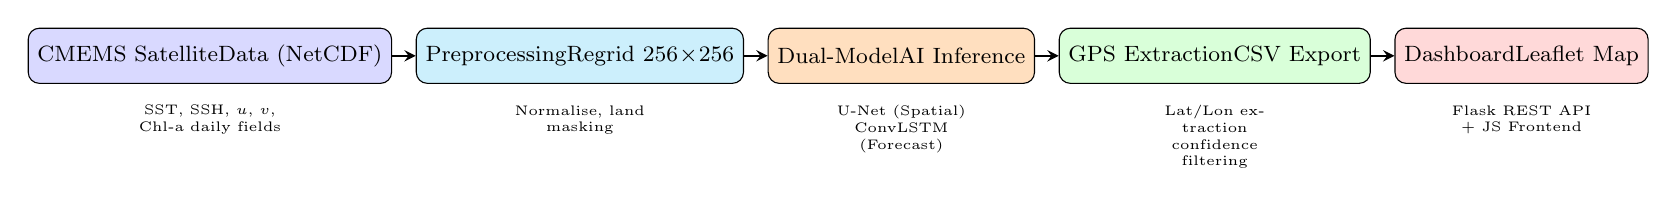
\begin{tikzpicture}[node distance=0.55cm, auto, font=\scriptsize]
  % Pipeline blocks
  \node[inputblock, minimum width=2.2cm](d1){CMEMS Satellite\\Data (NetCDF)};
  \node[encblock, right=0.3cm of d1, minimum width=2.2cm](d2){Preprocessing\\Regrid $256\!\times\!256$};
  \node[bottleneck, right=0.3cm of d2, minimum width=2.2cm](d3){Dual-Model\\AI Inference};
  \node[decblock, right=0.3cm of d3, minimum width=2.2cm](d4){GPS Extraction\\CSV Export};
  \node[outblock, right=0.3cm of d4, minimum width=2.2cm](d5){Dashboard\\Leaflet Map};

  \draw[arrow](d1)--(d2);
  \draw[arrow](d2)--(d3);
  \draw[arrow](d3)--(d4);
  \draw[arrow](d4)--(d5);

  % Sub-labels
  \node[below=0.15cm of d1, font=\tiny, text width=2cm, align=center]
    {SST, SSH, $u$, $v$,\\Chl-a daily fields};
  \node[below=0.15cm of d2, font=\tiny, text width=2cm, align=center]
    {Normalise, land\\masking};
  \node[below=0.15cm of d3, font=\tiny, text width=2cm, align=center]
    {U-Net (Spatial)\\ConvLSTM (Forecast)};
  \node[below=0.15cm of d4, font=\tiny, text width=2cm, align=center]
    {Lat/Lon extraction\\confidence filtering};
  \node[below=0.15cm of d5, font=\tiny, text width=2cm, align=center]
    {Flask REST API\\+ JS Frontend};
\end{tikzpicture}
\caption{PFZ Navigator end-to-end pipeline. Raw CMEMS satellite data
undergoes regridding before dual-model inference. Results are served
through a Flask API to an interactive Leaflet-based dashboard.}
\label{fig:pipeline}
\end{figure}

\subsection{U-Net Architecture for Spatial Segmentation}

Fig.~\ref{fig:unet_arch} presents the U-Net encoder-decoder
architecture with skip connections. Table~\ref{tab:unet_arch}
summarises the layer configuration.

\begin{figure}[htbp]
\centering
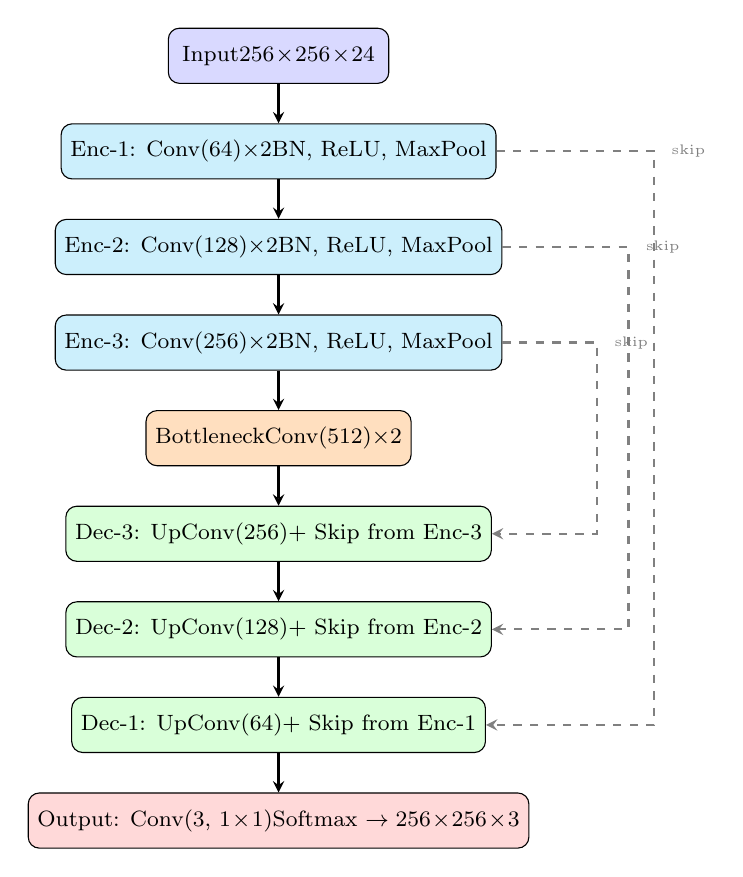
\begin{tikzpicture}[node distance=0.5cm, auto, font=\scriptsize]
  % Encoder
  \node[inputblock](in){Input\\$256\!\times\!256\!\times\!24$};
  \node[encblock, below=of in](e1){Enc-1: Conv(64)$\times$2\\
    BN, ReLU, MaxPool};
  \node[encblock, below=of e1](e2){Enc-2: Conv(128)$\times$2\\
    BN, ReLU, MaxPool};
  \node[encblock, below=of e2](e3){Enc-3: Conv(256)$\times$2\\
    BN, ReLU, MaxPool};
  \node[bottleneck, below=of e3](bn){Bottleneck\\Conv(512)$\times$2};
  % Decoder
  \node[decblock, below=of bn](d3){Dec-3: UpConv(256)\\+ Skip from Enc-3};
  \node[decblock, below=of d3](d2){Dec-2: UpConv(128)\\+ Skip from Enc-2};
  \node[decblock, below=of d2](d1){Dec-1: UpConv(64)\\+ Skip from Enc-1};
  \node[outblock, below=of d1](out){Output: Conv(3, $1\!\times\!1$)\\
    Softmax $\to 256\!\times\!256\!\times\!3$};

  % Main arrows
  \draw[arrow](in)--(e1);
  \draw[arrow](e1)--(e2);
  \draw[arrow](e2)--(e3);
  \draw[arrow](e3)--(bn);
  \draw[arrow](bn)--(d3);
  \draw[arrow](d3)--(d2);
  \draw[arrow](d2)--(d1);
  \draw[arrow](d1)--(out);

  % Skip connections
  \draw[skiparrow](e3.east) -- ++(1.2,0) |- (d3.east);
  \draw[skiparrow](e2.east) -- ++(1.6,0) |- (d2.east);
  \draw[skiparrow](e1.east) -- ++(2.0,0) |- (d1.east);

  % Skip labels
  \node[right=1.3cm of e3, font=\tiny, color=gray]{skip};
  \node[right=1.7cm of e2, font=\tiny, color=gray]{skip};
  \node[right=2.1cm of e1, font=\tiny, color=gray]{skip};
\end{tikzpicture}
\caption{U-Net encoder-decoder architecture with three encoder blocks,
a 512-channel bottleneck, three decoder blocks, and skip connections
(dashed arrows) preserving high-resolution spatial features.}
\label{fig:unet_arch}
\end{figure}

\begin{table}[htbp]
\caption{U-Net Layer Configuration}
\label{tab:unet_arch}
\centering
\footnotesize
\begin{tabular}{llc}
\toprule
\textbf{Block} & \textbf{Operations} & \textbf{Output Shape}\\
\midrule
Input      & ---                            & $256\!\times\!256\!\times\!24$\\
Enc-1      & Conv(64)$\times$2, BN, ReLU    & $128\!\times\!128\!\times\!64$\\
Enc-2      & Conv(128)$\times$2, BN, ReLU   & $64\!\times\!64\!\times\!128$\\
Enc-3      & Conv(256)$\times$2, BN, ReLU   & $32\!\times\!32\!\times\!256$\\
Bottleneck & Conv(512)$\times$2, BN, ReLU   & $32\!\times\!32\!\times\!512$\\
Dec-3      & UpConv(256) + Skip             & $64\!\times\!64\!\times\!256$\\
Dec-2      & UpConv(128) + Skip             & $128\!\times\!128\!\times\!128$\\
Dec-1      & UpConv(64) + Skip              & $256\!\times\!256\!\times\!64$\\
Output     & Conv(3, $1\!\times\!1$), Softmax & $256\!\times\!256\!\times\!3$\\
\bottomrule
\end{tabular}
\end{table}

\subsection{ConvLSTM Architecture for Spatio-Temporal Forecasting}

Fig.~\ref{fig:convlstm_arch} presents the ConvLSTM architecture.
Table~\ref{tab:convlstm_arch} details the layer configuration.

\begin{figure}[htbp]
\centering
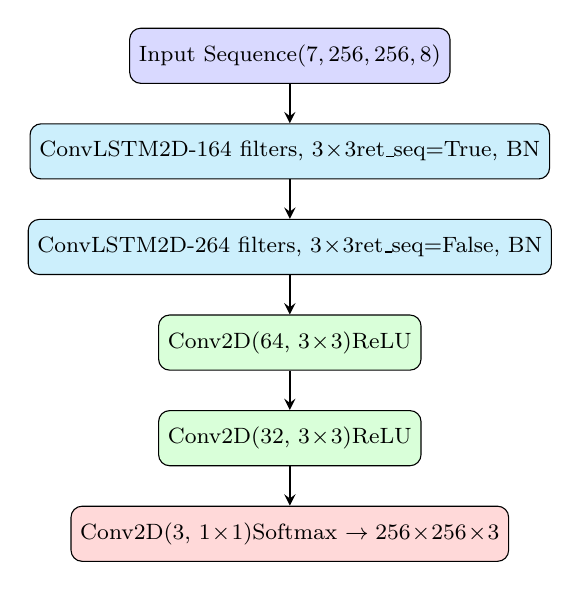
\begin{tikzpicture}[node distance=0.5cm, auto, font=\scriptsize]
  \node[inputblock](in){Input Sequence\\$(7, 256, 256, 8)$};
  \node[encblock, below=of in](c1){ConvLSTM2D-1\\64 filters, $3\!\times\!3$\\
    ret\_seq=True, BN};
  \node[encblock, below=of c1](c2){ConvLSTM2D-2\\64 filters, $3\!\times\!3$\\
    ret\_seq=False, BN};
  \node[decblock, below=of c2](cv1){Conv2D(64, $3\!\times\!3$)\\ReLU};
  \node[decblock, below=of cv1](cv2){Conv2D(32, $3\!\times\!3$)\\ReLU};
  \node[outblock, below=of cv2](out){Conv2D(3, $1\!\times\!1$)\\
    Softmax $\to 256\!\times\!256\!\times\!3$};

  \draw[arrow](in)--(c1);
  \draw[arrow](c1)--(c2);
  \draw[arrow](c2)--(cv1);
  \draw[arrow](cv1)--(cv2);
  \draw[arrow](cv2)--(out);
\end{tikzpicture}
\caption{ConvLSTM architecture for seven-day spatio-temporal forecasting.
The first ConvLSTM2D layer processes all 7 time steps; the second
collapses the sequence into a spatial representation decoded by Conv2D
layers into 3-class per-pixel probabilities.}
\label{fig:convlstm_arch}
\end{figure}

\begin{table}[htbp]
\caption{ConvLSTM Layer Configuration}
\label{tab:convlstm_arch}
\centering
\footnotesize
\begin{tabular}{llc}
\toprule
\textbf{Layer} & \textbf{Configuration} & \textbf{Output Shape}\\
\midrule
Input         & 7-frame sequence       & $(7, 256, 256, 8)$\\
ConvLSTM2D-1  & 64 filt., $3\!\times\!3$, seq & $(7, 256, 256, 64)$\\
ConvLSTM2D-2  & 64 filt., $3\!\times\!3$      & $(256, 256, 64)$\\
Conv2D-1      & 64 filt., $3\!\times\!3$, ReLU & $(256, 256, 64)$\\
Conv2D-2      & 32 filt., $3\!\times\!3$, ReLU & $(256, 256, 32)$\\
Output        & 3 filt., $1\!\times\!1$, Softmax & $(256, 256, 3)$\\
\bottomrule
\end{tabular}
\end{table}

The fundamental ConvLSTM cell operations are:
\begin{align}
\mathbf{i}_t &= \sigma\bigl(\mathbf{W}_{xi} * \mathbf{X}_t +
  \mathbf{W}_{hi} * \mathbf{H}_{t-1} + \mathbf{b}_i\bigr)
  \label{eq:input_gate}\\
\mathbf{f}_t &= \sigma\bigl(\mathbf{W}_{xf} * \mathbf{X}_t +
  \mathbf{W}_{hf} * \mathbf{H}_{t-1} + \mathbf{b}_f\bigr)
  \label{eq:forget_gate}\\
\mathbf{o}_t &= \sigma\bigl(\mathbf{W}_{xo} * \mathbf{X}_t +
  \mathbf{W}_{ho} * \mathbf{H}_{t-1} + \mathbf{b}_o\bigr)
  \label{eq:output_gate}\\
\tilde{\mathbf{C}}_t &= \tanh\bigl(\mathbf{W}_{xc} * \mathbf{X}_t +
  \mathbf{W}_{hc} * \mathbf{H}_{t-1} + \mathbf{b}_c\bigr)
  \label{eq:candidate}\\
\mathbf{C}_t &= \mathbf{f}_t \odot \mathbf{C}_{t-1} +
  \mathbf{i}_t \odot \tilde{\mathbf{C}}_t
  \label{eq:cell}\\
\mathbf{H}_t &= \mathbf{o}_t \odot \tanh(\mathbf{C}_t)
  \label{eq:hidden}
\end{align}
where $*$ denotes convolution, $\odot$ is Hadamard product, and
$\sigma$ is the sigmoid function.

% ============================================================
%             V. EXPERIMENTAL SETUP
% ============================================================
\section{Experimental Setup}

\subsection{Dataset: CMEMS Satellite Oceanography}
The dataset comprises daily satellite-derived ocean parameter fields
from the Copernicus Marine Environment Monitoring Service (CMEMS),
covering the Bay of Bengal study region ($5.0^\circ$--$14.5^\circ$N,
$77.0^\circ$--$84.92^\circ$E) over approximately eight years
(2016--2024), yielding $N = 2{,}914$ daily observations. Five
parameters are extracted: SST, SSH, $u$-velocity, $v$-velocity, and
Chlorophyll-a.

\subsection{Cross-Validation Protocols}

\subsubsection{Temporal Block CV (U-Net)}
The time series is partitioned into $k = 3$ non-overlapping contiguous
temporal blocks. In each fold, two blocks train the model and the
third is held out for validation. This prevents leakage from daily
auto-correlation.

\subsubsection{Walk-Forward Expanding Window CV (ConvLSTM)}
An expanding window protocol mirrors operational forecasting:
\begin{itemize}
    \item \textbf{Fold 1:} Train Years 1--3 $\to$ Validate Year 4
    \item \textbf{Fold 2:} Train Years 1--4 $\to$ Validate Year 5
    \item \textbf{Fold 3:} Train Years 1--5 $\to$ Validate Year 6
\end{itemize}

\subsection{Training Configuration}

\begin{table}[htbp]
\caption{Training Hyperparameters}
\label{tab:training_config}
\centering
\footnotesize
\begin{tabular}{lcc}
\toprule
\textbf{Parameter} & \textbf{U-Net} & \textbf{ConvLSTM}\\
\midrule
Optimiser              & Adam & Adam\\
Initial LR             & $1 \times 10^{-3}$ & $1 \times 10^{-3}$\\
Loss                   & Cat.\ Cross-Entropy & Cat.\ Cross-Entropy\\
Batch Size             & 8 & 4\\
Epochs per Fold        & 5 & 5\\
Input Shape            & $(256,256,24)$ & $(7,256,256,8)$\\
Output Shape           & $(256,256,3)$ & $(256,256,3)$\\
Output Activation      & Softmax & Softmax\\
CV Method              & Temporal Block & Walk-Forward\\
Folds ($k$)            & 3 & 3\\
\bottomrule
\end{tabular}
\end{table}

% ============================================================
%          VI. RESULTS AND DISCUSSION
% ============================================================
\section{Results and Discussion}

\subsection{U-Net Cross-Validation Results}

Table~\ref{tab:unet_cv} reports per-fold and aggregated metrics.
The U-Net achieves 92.13\% mean accuracy across three temporal folds
with a 95\% confidence interval of $\pm$0.017.

\begin{table}[htbp]
\caption{U-Net Temporal Block CV Results}
\label{tab:unet_cv}
\centering
\footnotesize
\begin{tabular}{lC{1cm}C{1cm}C{1cm}C{1.8cm}}
\toprule
\textbf{Metric} & \textbf{Fold\,1} & \textbf{Fold\,2} & \textbf{Fold\,3}
  & \textbf{Mean $\pm$ CI\textsubscript{95}}\\
\midrule
Accuracy      & 0.935 & 0.905 & 0.923 & 0.921 $\pm$ 0.017\\
Precision$_M$ & 0.936 & 0.869 & 0.930 & 0.911 $\pm$ 0.042\\
Recall$_M$    & 0.900 & 0.919 & 0.879 & 0.899 $\pm$ 0.023\\
F1$_M$        & 0.916 & 0.891 & 0.898 & 0.902 $\pm$ 0.015\\
$\kappa$      & 0.868 & 0.828 & 0.851 & 0.849 $\pm$ 0.023\\
mIoU          & 0.846 & 0.804 & 0.818 & 0.823 $\pm$ 0.024\\
\bottomrule
\end{tabular}
\end{table}

\subsection{U-Net Per-Class Analysis}

\begin{table}[htbp]
\caption{U-Net Per-Class Metrics (Mean $\pm$ Std)}
\label{tab:unet_perclass}
\centering
\footnotesize
\begin{tabular}{lcccc}
\toprule
\textbf{Class} & \textbf{Prec.} & \textbf{Rec.} & \textbf{F1}
  & \textbf{IoU}\\
\midrule
Low PFZ    & .890$\pm$.098 & .860$\pm$.117 & .866$\pm$.038 & .765$\pm$.059\\
Medium PFZ & .940$\pm$.016 & .940$\pm$.044 & .940$\pm$.015 & .887$\pm$.027\\
High PFZ   & .904$\pm$.048 & .898$\pm$.064 & .899$\pm$.017 & .817$\pm$.028\\
\bottomrule
\end{tabular}
\end{table}

\subsection{U-Net Confusion Matrix}

\begin{table}[htbp]
\caption{U-Net Aggregated Confusion Matrix (Normalised)}
\label{tab:unet_cm}
\centering
\begin{tabular}{lccc}
\toprule
& \multicolumn{3}{c}{\textbf{Predicted}} \\
\cmidrule(lr){2-4}
\textbf{True} & Low & Medium & High\\
\midrule
Low PFZ    & \textbf{0.861} & 0.130 & 0.009\\
Medium PFZ & 0.028 & \textbf{0.941} & 0.031\\
High PFZ   & 0.002 & 0.094 & \textbf{0.904}\\
\bottomrule
\end{tabular}
\end{table}

\subsection{U-Net Cross-Validation Plots}

Fig.~\ref{fig:unet_cv_plots} presents the six-panel publication-quality
cross-validation visualisations for the U-Net model.

\begin{figure}[htbp]
\centering
% ── PLACEHOLDER: uncomment when image is available ──
% \includegraphics[width=\linewidth]{cv_unet_temporal_block.png}
\fbox{\parbox{0.95\linewidth}{\centering\small\vspace{2cm}
  \textbf{[INSERT IMAGE: \texttt{cv\_unet\_temporal\_block.png}]}\\[6pt]
  6-panel plot containing:\\
  (1) Per-fold accuracy bar chart (mean = 0.9213)\\
  (2) Training \& validation learning curves (all folds)\\
  (3) Normalised aggregated confusion matrix\\
  (4) Per-class F1-score grouped bar chart\\
  (5) Radar chart of model performance metrics\\
  (6) Box-plot metric distributions across folds
\vspace{2cm}}}
\caption{U-Net Temporal Block cross-validation results. Six panels show
per-fold accuracy, learning curves, confusion matrix, per-class F1
scores, radar chart, and metric distribution box plots.}
\label{fig:unet_cv_plots}
\end{figure}

\subsection{ConvLSTM Cross-Validation Results}

\begin{table}[htbp]
\caption{ConvLSTM Walk-Forward CV Results}
\label{tab:lstm_cv}
\centering
\footnotesize
\begin{tabular}{lC{1cm}C{1cm}C{1cm}C{1.8cm}}
\toprule
\textbf{Metric} & \textbf{Fold\,1} & \textbf{Fold\,2} & \textbf{Fold\,3}
  & \textbf{Mean $\pm$ CI\textsubscript{95}}\\
\midrule
Accuracy      & 0.867 & 0.889 & 0.899 & 0.885 $\pm$ 0.019\\
Precision$_M$ & 0.874 & 0.884 & 0.909 & 0.889 $\pm$ 0.021\\
Recall$_M$    & 0.872 & 0.869 & 0.893 & 0.878 $\pm$ 0.015\\
F1$_M$        & 0.872 & 0.876 & 0.901 & 0.883 $\pm$ 0.018\\
$\kappa$      & 0.766 & 0.806 & 0.819 & 0.797 $\pm$ 0.031\\
mIoU          & 0.776 & 0.781 & 0.821 & 0.792 $\pm$ 0.028\\
\bottomrule
\end{tabular}
\end{table}

\subsection{ConvLSTM Per-Class Analysis}

\begin{table}[htbp]
\caption{ConvLSTM Per-Class Metrics (Mean $\pm$ Std)}
\label{tab:lstm_perclass}
\centering
\footnotesize
\begin{tabular}{lcccc}
\toprule
\textbf{Class} & \textbf{Prec.} & \textbf{Rec.} & \textbf{F1}
  & \textbf{IoU}\\
\midrule
Low PFZ    & .877$\pm$.027 & .829$\pm$.023 & .852$\pm$.024 & .743$\pm$.036\\
Medium PFZ & .915$\pm$.023 & .928$\pm$.021 & .921$\pm$.015 & .854$\pm$.026\\
High PFZ   & .874$\pm$.007 & .878$\pm$.015 & .876$\pm$.011 & .780$\pm$.017\\
\bottomrule
\end{tabular}
\end{table}

\subsection{ConvLSTM Confusion Matrix}

\begin{table}[htbp]
\caption{ConvLSTM Aggregated Confusion Matrix (Normalised)}
\label{tab:lstm_cm}
\centering
\begin{tabular}{lccc}
\toprule
& \multicolumn{3}{c}{\textbf{Predicted}} \\
\cmidrule(lr){2-4}
\textbf{True} & Low & Medium & High\\
\midrule
Low PFZ    & \textbf{0.830} & 0.136 & 0.034\\
Medium PFZ & 0.025 & \textbf{0.928} & 0.047\\
High PFZ   & 0.006 & 0.116 & \textbf{0.878}\\
\bottomrule
\end{tabular}
\end{table}

\subsection{ConvLSTM Cross-Validation Plots}

\begin{figure}[htbp]
\centering
% ── PLACEHOLDER: uncomment when image is available ──
% \includegraphics[width=\linewidth]{cv_convlstm_walk_forward.png}
\fbox{\parbox{0.95\linewidth}{\centering\small\vspace{2cm}
  \textbf{[INSERT IMAGE: \texttt{cv\_convlstm\_walk\_forward.png}]}\\[6pt]
  6-panel plot containing:\\
  (1) Per-fold accuracy bar chart (mean = 0.8849)\\
  (2) Training \& validation learning curves (all folds)\\
  (3) Normalised aggregated confusion matrix\\
  (4) Per-class F1-score grouped bar chart\\
  (5) Radar chart of model performance metrics\\
  (6) Box-plot metric distributions across folds
\vspace{2cm}}}
\caption{ConvLSTM Walk-Forward cross-validation results. Six panels
show per-fold accuracy, learning curves, confusion matrix, per-class
F1 scores, radar chart, and metric distribution box plots.}
\label{fig:convlstm_cv_plots}
\end{figure}

\subsection{Comparative Benchmark: U-Net vs.\ ConvLSTM}

Table~\ref{tab:comparison} provides a direct comparison between the
two models.

\begin{table}[htbp]
\caption{Model Comparison: U-Net (Spatial) vs.\ ConvLSTM (Temporal)}
\label{tab:comparison}
\centering
\footnotesize
\begin{tabular}{lccc}
\toprule
\textbf{Metric} & \textbf{U-Net} & \textbf{ConvLSTM} & $\boldsymbol{\Delta}$\\
\midrule
Accuracy           & \textbf{92.13\%} & 88.49\% & +3.64\%\\
Macro Precision    & \textbf{91.15\%} & 88.90\% & +2.25\%\\
Macro Recall       & \textbf{89.94\%} & 87.82\% & +2.12\%\\
Macro F1           & \textbf{90.16\%} & 88.32\% & +1.84\%\\
Cohen's $\kappa$   & \textbf{0.849}   & 0.797   & +0.052\\
mIoU               & \textbf{82.29\%} & 79.24\% & +3.05\%\\
\midrule
Task               & Nowcasting  & Forecasting & ---\\
Input Shape        & $(256,256,24)$ & $(7,256,256,8)$ & ---\\
CV Method          & Temp.\ Block & Walk-Forward & ---\\
\bottomrule
\end{tabular}
\end{table}

The U-Net outperforms ConvLSTM on all metrics, consistent with
the inherent difficulty difference: spatial analysis of the present
state is easier than temporal extrapolation. The modest 3.64
percentage point accuracy gap confirms that the ConvLSTM provides
operationally useful seven-day forecasts despite the increased task
complexity.

\subsection{Dashboard Output Screenshots}

\begin{figure}[htbp]
\centering
% ── PLACEHOLDER ──
\fbox{\parbox{0.95\linewidth}{\centering\small\vspace{1.5cm}
  \textbf{[INSERT IMAGE: Dashboard main page screenshot]}\\[6pt]
  Shows: PFZ Navigator dashboard with navigation sidebar (Dashboard,
  Predict, Forecast, Live Map, Analytics, Research, Upload), stat
  cards displaying U-Net and ConvLSTM accuracy, training history
  charts, and system status indicators.
\vspace{1.5cm}}}
\caption{PFZ Navigator dashboard main page showing system status,
model accuracy statistics, and training history visualisations.}
\label{fig:dashboard}
\end{figure}

\begin{figure}[htbp]
\centering
% ── PLACEHOLDER ──
\fbox{\parbox{0.95\linewidth}{\centering\small\vspace{1.5cm}
  \textbf{[INSERT IMAGE: U-Net prediction output map]}\\[6pt]
  Shows: Two-panel PFZ map --- left panel displays 3-class colour-coded
  PFZ classification (blue=Low, amber=Medium, red=High); right panel
  shows high-PFZ confidence heatmap. Includes GPS coordinate table
  below.
\vspace{1.5cm}}}
\caption{U-Net prediction output: PFZ classification map (left) and
high-PFZ confidence score heatmap (right), with top-20 GPS
coordinates extracted for the date 2018-04-11.}
\label{fig:unet_output}
\end{figure}

\begin{figure}[htbp]
\centering
% ── PLACEHOLDER ──
\fbox{\parbox{0.95\linewidth}{\centering\small\vspace{1.5cm}
  \textbf{[INSERT IMAGE: Live Map Leaflet screenshot]}\\[6pt]
  Shows: Interactive Leaflet map displaying PFZ heatmap overlay on
  Tamil Nadu coast with real-world geography (cities visible:
  Thoothukudi, Madurai, Jaffna). Red GPS markers on high-PFZ zones.
  Legend: Low PFZ (blue), Medium PFZ (amber), High PFZ (red).
\vspace{1.5cm}}}
\caption{Live interactive PFZ map rendered via Leaflet. The AI-
generated heatmap is geographically overlaid on the Tamil Nadu
coast with automatic GPS markers on high-PFZ zones.}
\label{fig:livemap}
\end{figure}

\subsection{GPS Coordinate Extraction}

The system converts pixel-level High PFZ predictions into geographic
coordinates:
\begin{align}
\text{lat}_{i} &= \phi_{\min} + i \cdot
  \frac{\phi_{\max} - \phi_{\min}}{H}
  \label{eq:lat}\\
\text{lon}_{j} &= \lambda_{\min} + j \cdot
  \frac{\lambda_{\max} - \lambda_{\min}}{W}
  \label{eq:lon}
\end{align}
Points are filtered by a confidence threshold (default 60\%), sorted
by descending confidence, and exported as downloadable CSV files for
maritime GPS navigation systems.

% ============================================================
%         VII. CONCLUSION AND FUTURE WORK
% ============================================================
\section{Conclusion and Future Work}

This paper presented PFZ Navigator, an end-to-end deep learning
system for identifying and forecasting Potential Fishing Zones in the
Bay of Bengal. The dual-model architecture integrates a U-Net for
high-resolution spatial segmentation (92.13\% accuracy, 0.940~F1 for
Medium PFZ, 0.899~F1 for High PFZ) and a ConvLSTM for seven-day
spatio-temporal forecasting (88.49\% accuracy, 0.921~F1 for Medium
PFZ, 0.876~F1 for High PFZ). Both models are rigorously validated
through temporally separated cross-validation protocols.

The system is deployed as a full-stack web application with real-time
inference, interactive Leaflet geographic visualisation, and automated
GPS coordinate extraction. The work directly addresses SDG-14 (Life
Below Water) by enabling data-driven sustainable fishing practices.

Future directions include: (1)~higher-resolution satellite inputs
(Sentinel-3 OLCI at 300~m), (2)~attention-augmented U-Net and
Transformer-based forecasting, (3)~automated daily CMEMS data
ingestion via scheduled FTP, (4)~mobile deployment with offline
inference, (5)~multi-species PFZ models trained on catch records, and
(6)~seasonal and monsoon-specific feature engineering.

% ============================================================
%                    REFERENCES
% ============================================================
\begin{thebibliography}{20}

\bibitem{solanki2003}
H.~U.~Solanki, R.~M.~Dwivedi, S.~R.~Nayak, V.~S.~Somvanshi,
D.~K.~Gulati, and S.~K.~Pattnayak, ``Application of ocean colour
monitor chlorophyll and AVHRR SST for fishery forecast: Preliminary
validation results off Gujarat coast, northwest coast of India,''
\emph{Indian J.\ Mar.\ Sci.}, vol.~32, no.~3, pp.~245--252,
Sep.~2003.

\bibitem{tang2003}
D.~L.~Tang, I.~H.~Ni, D.~R.~Kester, and F.~E.~M{\"u}ller-Karger,
``Remote sensing observations of winter phytoplankton blooms southwest
of the Luzon strait in the South China Sea,'' \emph{Mar.\ Ecol.\
Prog.\ Ser.}, vol.~261, pp.~65--75, 2003.

\bibitem{zhang_ensemble2023}
Y.~Zhang, H.~Liu, and W.~Chen, ``Prediction of potential fishing zones
using ensemble machine learning models on multi-parameter oceanographic
satellite data,'' \emph{Ocean Engineering}, vol.~275, Art.~no.~114130,
May~2023.

\bibitem{fitrianah2015}
D.~Fitrianah, A.~N.~Hidayanto, H.~Fahmi, J.~K.~Lumban Gaol, and
A.~M.~Arymurthy, ``ST-AGRID: A spatio temporal grid density based
clustering and its application for determining potential fishing
zone,'' \emph{IEEE J.\ Sel.\ Topics Appl.\ Earth Observ.\ Remote
Sens.\ (JSTARS)}, vol.~8, no.~2, pp.~619--629, Feb.~2015.

\bibitem{fitrianah_feature2016}
D.~Fitrianah, H.~Fahmi, A.~N.~Hidayanto, and A.~M.~Arymurthy,
``Feature exploration for prediction of potential fishing zones from
remote sensing satellite,'' \emph{Int.\ J.\ Inf.\ Technol.\ Comput.\
Sci.}, vol.~8, no.~3, pp.~38--45, Mar.~2016.

\bibitem{sivasankari2022}
V.~Sivasankari, K.~Mahalakshmi, and M.~S.~Kavitha, ``HE-DFNETS: Hybrid
ensemble deep feature networks for identifying potential fishing zones
from satellite imagery,'' \emph{Comput.\ Intell.\ Neurosci.},
vol.~2022, Art.~no.~4825035, 2022.

\bibitem{vinston2023}
R.~Vinston~Raja, A.~Sundarambal, and S.~Maheswari, ``Forecasting of
potential fishing zones using function fitting neural network and
multi-parameter oceanographic satellite data,'' \emph{J.\ Mar.\ Sci.\
Technol.}, vol.~28, no.~1, pp.~105--119, Mar.~2023.

\bibitem{yaacob2024}
R.~Ya'acob, N.~Z.~Azmi, N.~S.~Nadia, and S.~S.~S.~Ahmad, ``A review
on potential fishing zone prediction using machine learning and deep
learning approaches,'' \emph{Artif.\ Intell.\ Rev.}, vol.~57,
Art.~no.~48, Jan.~2024.

\bibitem{janani2025}
T.~Janani, R.~Selvakumar, and P.~Sathish~Kumar, ``Identification of
potential fishing zones using multi-parameter satellite data with
clustering and ensemble classification,'' \emph{Remote Sens.\ Appl.\
Soc.\ Environ.}, vol.~37, Art.~no.~101133, Jan.~2025.

\bibitem{ronneberger2015}
O.~Ronneberger, P.~Fischer, and T.~Brox, ``U-Net: Convolutional
networks for biomedical image segmentation,'' in \emph{Proc.\ MICCAI},
Munich, Germany, Oct.~2015, pp.~234--241.

\bibitem{shi2015}
X.~Shi, Z.~Chen, H.~Wang, D.~Y.~Yeung, W.~K.~Wong, and W.~C.~Woo,
``Convolutional LSTM network: A machine learning approach for
precipitation nowcasting,'' in \emph{Proc.\ NeurIPS}, Montr\'{e}al,
Canada, Dec.~2015, pp.~802--810.

\bibitem{hochreiter1997}
S.~Hochreiter and J.~Schmidhuber, ``Long short-term memory,''
\emph{Neural Comput.}, vol.~9, no.~8, pp.~1735--1780, Nov.~1997.

\bibitem{lecun2015}
Y.~LeCun, Y.~Bengio, and G.~Hinton, ``Deep learning,'' \emph{Nature},
vol.~521, no.~7553, pp.~436--444, May~2015.

\bibitem{zhang_unet2018}
P.~Zhang, Y.~Ke, Z.~Zhang, M.~Wang, P.~Li, and S.~Zhang, ``Urban land
use and land cover classification using novel deep learning models
based on high spatial resolution satellite imagery,'' \emph{Sensors},
vol.~18, no.~11, Art.~no.~3717, Oct.~2018.

\bibitem{ham2019}
Y.~G.~Ham, J.~H.~Kim, and J.~J.~Luo, ``Deep learning for multi-year
ENSO forecasts,'' \emph{Nature}, vol.~573, no.~7775, pp.~568--572,
Sep.~2019.

\bibitem{he2016}
K.~He, X.~Zhang, S.~Ren, and J.~Sun, ``Deep residual learning for
image recognition,'' in \emph{Proc.\ IEEE CVPR}, Las Vegas, NV,
Jun.~2016, pp.~770--778.

\bibitem{ioffe2015}
S.~Ioffe and C.~Szegedy, ``Batch normalization: Accelerating deep
network training by reducing internal covariate shift,'' in
\emph{Proc.\ ICML}, Lille, France, Jul.~2015, pp.~448--456.

\end{thebibliography}

\end{document}